\documentclass[10pt,a4paper]{article}

\usepackage[T1]{fontenc}
\usepackage{lmodern}
\usepackage[protrusion=true,expansion=true]{microtype}
\usepackage[left=13mm,right=13mm,top=12mm,bottom=12mm]{geometry}
\usepackage{xcolor}
\usepackage{tabularx}
\usepackage{enumitem}
\usepackage{tikz}
\usetikzlibrary{arrows.meta,positioning}

\definecolor{PitchNavy}{HTML}{17324D}
\definecolor{PitchTeal}{HTML}{007C83}
\definecolor{PitchPale}{HTML}{EAF4F4}
\definecolor{PitchGrey}{HTML}{52616B}
\definecolor{PitchRule}{HTML}{CAD6DC}

\pagestyle{empty}
\setlength{\parindent}{0pt}
\setlength{\parskip}{2.6pt}
\setlist[itemize]{leftmargin=3.8mm,itemsep=1.2pt,topsep=1.8pt,parsep=0pt,partopsep=0pt}
\newcommand{\sectiontitle}[1]{%
  {\color{PitchTeal}\bfseries\fontsize{12.2}{13.2}\selectfont #1}\par
  \vspace{1.3pt}{\color{PitchRule}\rule{\linewidth}{0.45pt}}\vspace{2.2pt}%
}
\newcommand{\smalllabel}[1]{%
  {\color{PitchTeal}\bfseries\fontsize{8.3}{9.2}\selectfont\MakeUppercase{#1}}%
}

\begin{document}
\fontsize{9.2}{11.0}\selectfont
\raggedright

\colorbox{PitchNavy}{%
  \parbox{\dimexpr\linewidth-2\fboxsep\relax}{%
    \vspace{3.2mm}
    {\color{white}\bfseries\fontsize{8.3}{9.2}\selectfont\MakeUppercase{BMEG3920 Engineering Prototype}}\par
    \vspace{1.2mm}
    {\color{white}\bfseries\fontsize{27}{29}\selectfont LiteRehab Fusion}\par
    \vspace{1.2mm}
    {\color{white}\fontsize{12.4}{14.2}\selectfont Real-time guidance for more consistent upper-limb rehabilitation practice at home.}\par
    \vspace{3.2mm}
  }%
}

\vspace{4.2mm}

\begin{minipage}[t]{0.485\linewidth}
  \vspace{0pt}\raggedright
  \sectiontitle{The gap}
  A patient can leave a physiotherapy appointment knowing which exercises to practise. At home, the harder question is whether each repetition is controlled, large enough, or being completed by leaning the trunk. Useful feedback may not arrive until the next appointment, after the practice has already happened.
\end{minipage}\hfill
{\color{PitchRule}\vrule width 0.5pt}\hfill
\begin{minipage}[t]{0.485\linewidth}
  \vspace{0pt}\raggedright
  \sectiontitle{Our response}
  LiteRehab Fusion gives feedback while the exercise is happening. The wearable and camera-based prototype identifies the demonstrated movement, counts repetitions, flags common practice errors, and records the session for later review.
\end{minipage}

\vspace{4.0mm}
\sectiontitle{How it works}

\begin{center}
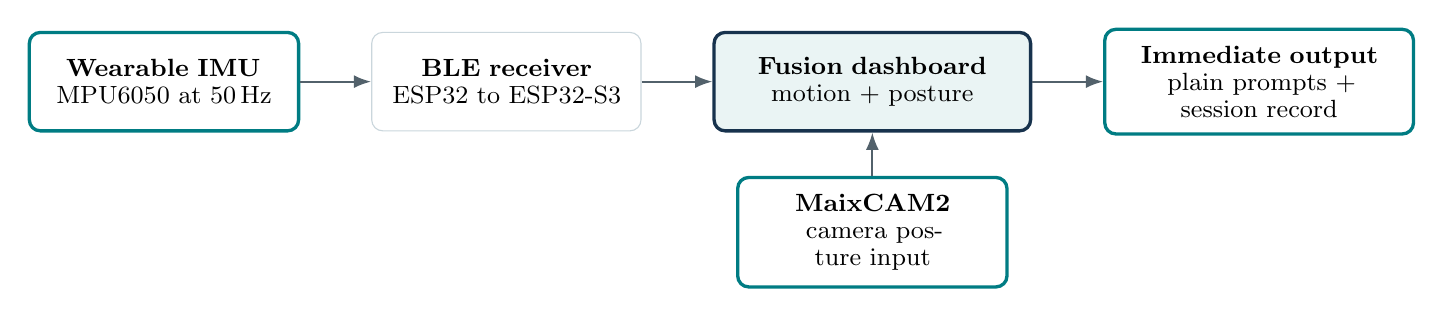
\begin{tikzpicture}[
  node distance=7.5mm and 9mm,
  box/.style={draw=PitchRule,fill=white,rounded corners=1.4mm,minimum height=12.5mm,text width=30mm,align=center,inner sep=2.1mm,font=\fontsize{8.7}{9.8}\selectfont},
  input/.style={box,draw=PitchTeal,very thick},
  core/.style={box,draw=PitchNavy,very thick,fill=PitchPale,text width=36mm},
  output/.style={box,draw=PitchTeal,very thick,text width=35mm},
  arrow/.style={-{Latex[length=2.2mm]},line width=0.75pt,draw=PitchGrey}
]
  \node[input] (imu) {\textbf{Wearable IMU}\\MPU6050 at 50\,Hz};
  \node[box,right=of imu] (ble) {\textbf{BLE receiver}\\ESP32 to ESP32-S3};
  \node[core,right=of ble] (dash) {\textbf{Fusion dashboard}\\motion + posture};
  \node[output,right=of dash] (out) {\textbf{Immediate output}\\plain prompts + session record};
  \node[input,below=5.5mm of dash] (cam) {\textbf{MaixCAM2}\\camera posture input};
  \draw[arrow] (imu) -- (ble);
  \draw[arrow] (ble) -- (dash);
  \draw[arrow] (cam) -- (dash);
  \draw[arrow] (dash) -- (out);
\end{tikzpicture}
\end{center}

\vspace{1.0mm}
\begin{minipage}[t]{0.61\linewidth}
  \vspace{0pt}\raggedright
  \sectiontitle{What the MVP demonstrates}
  \begin{itemize}
    \item Recognises the demonstrated elbow flexion and forearm rotation exercises.
    \item Gives immediate feedback for excessive speed, insufficient range, and trunk compensation.
    \item Shows repetition count on the wearable, with local LED and buzzer feedback.
    \item Keeps a synchronized record of IMU and pose information.
    \item Runs a classroom CNN-BiGRU baseline with a rule-based fallback.
    \item Passes \textbf{70 Python tests}, \textbf{three C host tests}, a model-loading smoke test, and builds for both ESP32 targets.
  \end{itemize}
\end{minipage}\hfill
{\color{PitchRule}\vrule width 0.5pt}\hfill
\begin{minipage}[t]{0.355\linewidth}
  \vspace{0pt}\raggedright
  \sectiontitle{Who benefits}
  \smalllabel{Patient}\par
  A clear cue arrives during the repetition instead of days later.

  \vspace{2.5mm}
  \smalllabel{Physiotherapist}\par
  A session record could show what happened between appointments, while the physiotherapist keeps responsibility for exercise selection and clinical decisions.
\end{minipage}

\vspace{3.6mm}

\begin{minipage}[t]{0.485\linewidth}
  \vspace{0pt}\raggedright
  \sectiontitle{Route to use}
  The proposed first step is a supervised pilot with physiotherapists. A later version could be supplied through rehabilitation providers as part of a prescribed home-exercise programme. The physiotherapist would choose the exercises and review the records.
\end{minipage}\hfill
{\color{PitchRule}\vrule width 0.5pt}\hfill
\begin{minipage}[t]{0.485\linewidth}
  \vspace{0pt}\raggedright
  \sectiontitle{Current limits}
  LiteRehab Fusion is an engineering prototype, \textbf{not a medical device}. It does not diagnose, prescribe treatment, score recovery, or replace professional supervision. The current model uses a small public dataset, supports a limited exercise set, and makes no clinical accuracy claim.
\end{minipage}

\vfill

\colorbox{PitchPale}{%
  \parbox{\dimexpr\linewidth-2\fboxsep\relax}{%
    \vspace{2.3mm}
    {\color{PitchTeal}\bfseries\fontsize{11.2}{12.6}\selectfont What we need next}\par
    \vspace{0.7mm}
    We are looking for physiotherapist partners to test usability, refine the feedback, and collect representative movement data under professional supervision.
    \vspace{2.3mm}
  }%
}

\end{document}
